\chapter{Binned analysis: Developing a new technique focused on background reduction}
\label{analysis}

\gls{anita} is a NASA long-duration balloon experiment for the detection of \gls{uhe} ($>10^{18}\,\mbox{eV}$) neutrinos. 
In this chapter, we present details of the development of a new technique for analysis using data collected during the second and third flights of \gls{anita}.
The approach used in this new technique is to section off the Antarctic ice
into bins and perform a search with different thresholds in each bin.  This new strategy was tested on data from the second flight of \gls{anita} which took place in $2008 - 2009$~\cite{brianDaileyThesis} before being used to search for neutrinos in data from the \gls{anita}-3 flight which took place in $2014 - 2015$~\cite{samStaffordThesis,jacobGordonThesis}.
This ``binned analysis'' is complementary to other \gls{anita} analyses that are centered around clustering of events on the continent.

\section{Searching for Neutrinos with ANITA}
With 48 dual-polarized, horn antennas on-board, \gls{anita} looks for the Askaryan radio signature of \gls{uhe} neutrinos in the $200 - 1200\,\mbox{MHz}$ band.  
\gls{anita} has a three-level trigger that 
requires excursions in power over thermal noise expectations with relative delays that are 
consistent with what is expected from a plane wave incident on the payload.
\gls{anita} records ``events'' as $100\,\mbox{ns}$-long
voltage waveforms from each polarization of each antenna, sampled at 2.6~GHz.

\subsection{Motivation}
\label{motivation}

Searches for \gls{uhe} neutrinos in the \gls{anita} data are conducted following a couple of different techniques. 
Traditionally, searches have used methods centered around event clustering, henceforth referred to as clustering analyses. After selecting for events with high signal-to-noise ratios that reconstruct to the continent, these analyses search for events that do not cluster with other events and whose reconstructed place of origin on the ice are not consistent with any known bases or locations of known human activity.  
In the searches for a diffuse flux of \gls{uhe} neutrinos in data collected during the \gls{anita}-1 flight in $2006 - 2007$ and the \gls{anita}-2 flight in $2008 - 2009$, as presented in~\cite{anita1} and~\cite{anita2} respectively, in the absence of signal, we placed the strongest limits on the flux of cosmic neutrinos in the $10^{18} - 10^{21} \,\mbox{eV}$ energy regime.
The analysis presented in this chapter uses a different ``binned'' approach and complements the clustering analyses in terms of its sensitivity  to neutrinos in different regions of ice.

The motivation behind the binned analysis is to maintain 
sensitivity for neutrinos even in regions of ice where
sources of anthropogenic noise are present.
In the clustering analysis, a neutrino candidate would be 
in the form of a ``non-base singlet'' or an event that would pass what is known as the ``clustering cut.'' A clustering cut attempts to remove anthropogenic backgrounds by eliminating all events that are less than a certain minimum distance away from any bases and/or ``hot spots" of human activity as well as from any other events that passed all other cuts. In a clustering analysis, regions of ice near other high SNR, reconstructing events or near regions of human activity are removed from the search.  The binned analysis instead attempts to use all of the ice, and searches for events that stand out among other events that reconstruct to the same region.

Figure~\ref{ben_clustering} shows the area of ice used
for neutrino searching in one of the two independent clustering analyses of the \gls{anita}-3 data~\cite{diffuse}. The red points in the figure denote simulated neutrinos that fail the clustering cut while the blue points denote those that pass. 
Here, neutrinos are simulated using the Kotera model flux~\cite{kotera}.
As seen in Figure~\ref{ben_clustering}, the 
clustering cut removes regions of ice and results in losses in sensitivity to a cosmogenic neutrino flux. 
We attempt to recover part of this sensitivity in the binned analysis. 
In this chapter, we present the binned analysis strategy 
and methods with a focus on background reduction. The work shown here is built upon modules completed by other binned analysts as are detailed in their theses ~\cite{brianDaileyThesis,samStaffordThesis,jacobGordonThesis}.

\begin{figure}
\centering
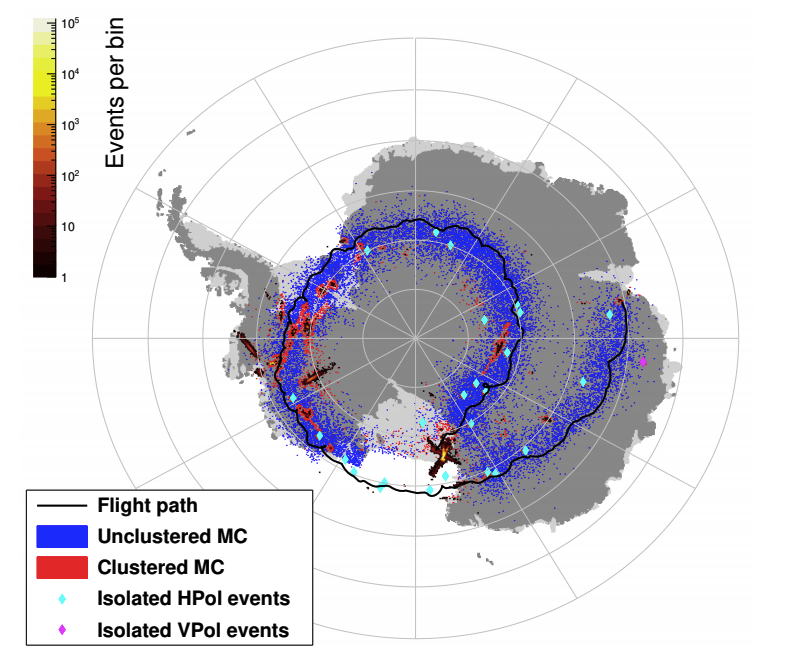
\includegraphics[width=1.0\textwidth]{figures/ben_clustering.png}
\caption{This is a figure from the clustering analysis performed by Ben Strutt during his postdoc at UCLA~\cite{diffuse}. Blue points represent simulated neutrinos that pass the clustering cut, while red points indicate ones that fail. The teal points show candidates of extensive air showers. The single pink point shows the neutrino candidate from this analysis.}
\label{ben_clustering}
\end{figure}

\section{Binned analysis approach} 

In the binned analysis, the Antarctic ice observed by the \gls{anita} payload is sectioned off into bins of nearly equal area.  
For this we use the Healpix package~\cite{healpix}, 
normally used to bin the sky for use
in cosmology, but here it is used to bin the earth.
Figure~\ref{bins} shows Healpix binning for the \gls{anita}-2 and -3 binned analyses where the coordinate
system is centered at the South Pole.
We overlay an outline of the continent of Antarctica and 
the flight path for the particular flight. The binned approach attempts to maintain the ability to search for neutrinos in as many bins as possible where we are sensitive.  

Figure~\ref{anita2bins} shows simulated neutrinos as reconstructing to different bins in the \gls{anita}-2 binned analysis. The color in these bins is representative of \gls{anita}'s sensitivity to neutrinos in that bin where sensitivity is in arbitrary units. It can be seen that the sensitivity to neutrinos varies bin to bin. Some parts of the continent have larger ice depth than others, and typically, \gls{anita} is more sensitive to neutrinos in these parts. 

Figure~\ref{anita3bins} shows events from the 10\% data before final cuts as reconstructing to different bins in the \gls{anita}-3 binned analysis. 
These events are dominated by noise. In \gls{anita}, noise events are mainly either due to thermal radiation from the ice or from human activities. It can be seen that some bins have more events than others as indicated by the color in that bin. This is mainly because some parts of the continent have more human activity than others. In other words, in some bins the anthropogenic backgrounds are larger than others, 
and in those bins we will need a higher 
threshold for our analysis cuts than those bins where
the events that reconstruct there are
predominantly triggered due to thermal noise fluctuations. Figure~\ref{a2_efficiency} shows the efficiency as a function of SNR in the ANITA-2 binned analysis.

\begin{figure}
\centering
\subfloat[ANITA-2 simulated neutrinos showing sensitivity in different bins]{
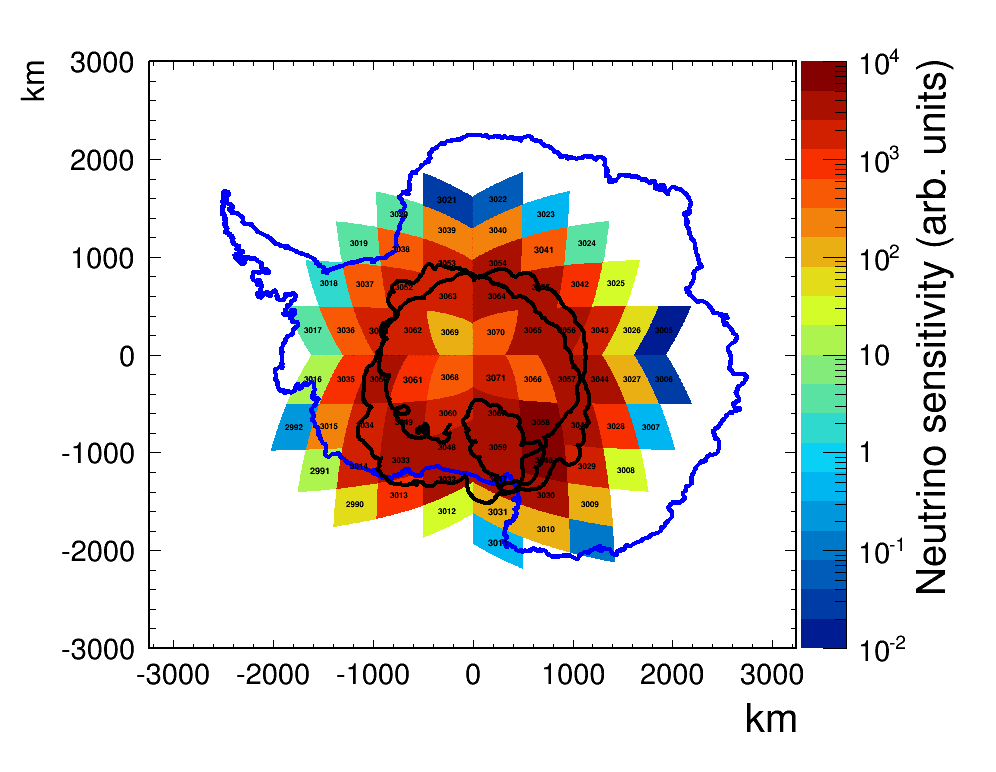
\includegraphics[width=0.72 \textwidth]{figures/healPixMapSimFinal.png}
\label{anita2bins}
} \par
\subfloat[ANITA-3 10\% data showing noise levels in different bins]{
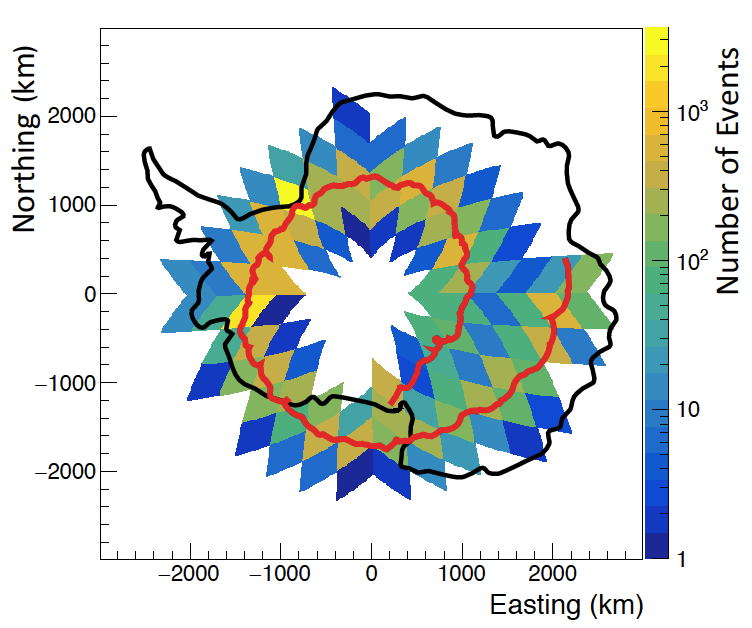
\includegraphics[width=0.72 \textwidth]{figures/binned.png}
\label{anita3bins}
}
\caption{Top: Simulated neutrinos in the ANITA-2 flight. Bottom: 10\% data before final cuts in the ANITA-3 flight. In both plots, color represents the number of events in that bin. An outline of Antarctica and the flight path are overlaid. It can be seen from the top plot that the sensitivity to neutrinos is different in different bins. Typically, sensitivity is larger in parts of the continent with greater ice depth.}
\label{bins}
\end{figure}

\subsection{Bins and event weights}

One of the features of the binned analysis is that we sort events into different bins.  The bin in which an event falls is determined by tracing its reconstruction direction back to the surface of Antarctica.  Using functions written in the \gls{anita} analysis tools by Ryan Nichol, and BEDMAP2, a dataset of the surface elevation of Antarctica, the location at which the event came out of the ice is found.  This location in longitude and latitude can be used to locate which Healpix bin an event falls in.  Events that are very close to the boundary between bins are assigned a weight based on how much of a one-standard-deviation error ellipse around the event, based on uncertainty in the event's reconstructed angels, is inside of the bin.  Events that fall entirely inside of one bin have a weight of one. 

\subsection{Blinding}

\gls{anita} uses blinding strategies to ensure that analyzers do not know which events will 
be considered candidates while they are designing cuts.  Blinding approaches have    
varied among different \gls{anita} analyses, and are briefly summarized here. 

Beginning with \gls{anita}-2, each ANITA data set has been ``salted'' with an unknown 
number (on order a few) fake candidates.  These are calibration pulser events whose origin on the continent have been scrambled.  Once final cuts have been imposed, these so-called inserted events are removed.

The published \gls{anita}-2 clustering analysis, presented in~\cite{anita2}, also used an ``ABCD'' approach where we categorized events according to how they clustered with other events, and stayed blind to events that were isolated from other events and from other bases until the final step before removing inserted events.  The ABCD refers to four different categories of clusters:  multiplets associated with bases (base clusters), singlets associated with bases (base singlets), multiplets that are not associated with bases (non-base clusters), and the blinded non-base singlets.

In the binned analysis presented here, in addition to salting, we use 10\% of the dataset (the burn sample) for understanding backgrounds and setting cuts, while being blind to the remaining 90\% of the data until the final step where we impose cuts on the 90\% set to identify candidates. 

\begin{figure}
\centering
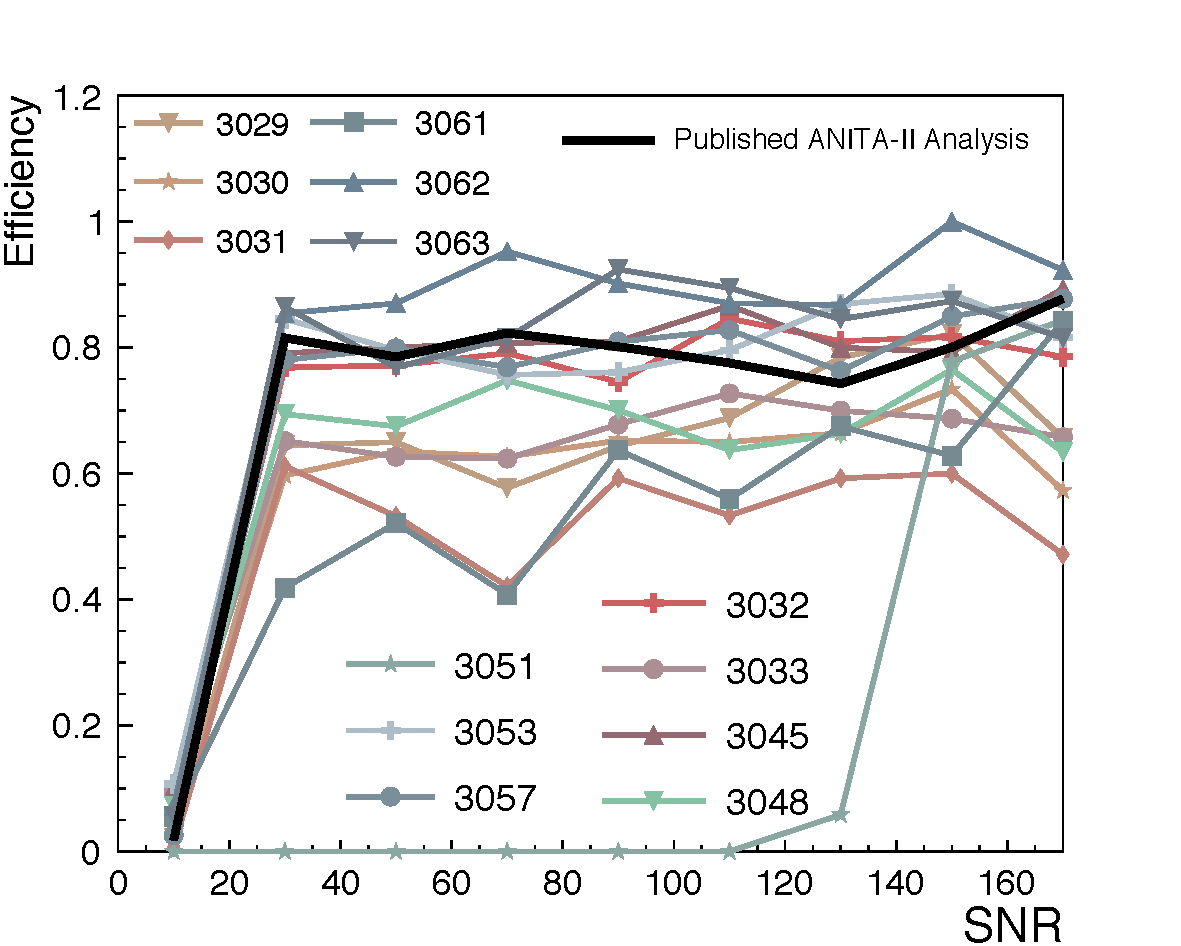
\includegraphics[width=0.7\textwidth]{figures/efficiencyA2_2.pdf}
\caption{Efficiency as a function of SNR in the ANITA-2 binned analysis. The solid, black line shows the efficiency for the ANITA-2 clustering analysis~\cite{anita2}. While the clustering analysis would have a single curve for efficiency, the binned analysis has such a curve in each bin kept in the analysis.}
\label{a2_efficiency}
\end{figure}

\section{Background reduction}
\label{background}

The \gls{anita} experiment records millions of events, most of which are noise. Eight, 26, 80, and 97 million events were recorded in the \gls{anita}-1, -2, -3, and -4 flights, respectively. 
As \gls{uhe} neutrino hunters, we are looking for extremely rare events in the \gls{anita} data. The name of the game, therefore, is to remove noise from the data or apply ``cuts". Cuts are roughly categorized as quality, analysis and final analysis cuts.
To give an idea, this is briefly described for the \gls{anita}-3 binned analysis in the following subsections. Details on cuts can also be found in~\cite{brianDaileyThesis,samStaffordThesis,jacobGordonThesis}. 


\subsection{Quality cuts}
\label{qcuts}

The first stage of cuts made are known as quality cuts.
These cuts mainly remove events that do not meet basic standards involving the trigger and digitizer. We also try to remove noise events caused by the payload itself in this phase of the analysis.  
\subsubsection{No Trigger Cut}

The No Trigger Cut requires the recorded event to have a triggering phi sector.  If the event did not cause a phi sector to trigger, then it is cut.

\subsubsection{Trigger Type Cut}

This cut requires the trigger type to be a radio frequency (RF) trigger.   Events that are not RF triggers are cut.
 
\subsubsection{SURF Saturation Cut}

The SURF's operating range only extends up to 1.5 V.  If an event's waveform goes beyond that operating range, it can become distorted.  Due to this, events with more than three waveforms that exceed 1.5 V are cut.

\subsubsection{DC Offset Cut}

Some events have waveforms with noticeable DC offsets.  This is thought to be due to digitization problems.  If an event has a mean value in their waveform of greater than 100 mV in any channel, it is cut.  

\subsubsection{Short-trace Cut}

A complete waveform in \gls{anita}-3 has 240 data entries or samples.  If an event has less than 240 samples for any reason, it is considered incomplete and cut.

\subsubsection{Payload Blast Cut}

Payload blast events are events that appear to be coming from the payload itself.  They are both impulsive and often have a high SNR. Because of these features, payload blast events can be quite problematic to our analysis.  Both this cut and the nadir noise events cut are designed to remove payload blast events.  This cut removes events that have an L3 trigger across 6 or more phi sectors.  Payload blasts are able to trigger many channels.  

\subsubsection{Nadir Noise Cut}

The peak voltages in the bottom ring antennas of payload blast events are dramatically larger than the peak voltages in the top ring. This cut is designed based on this feature.  
If the maximum peak voltage in the top ring is less than one half the maximum peak voltage in the bottom ring, the event is cut. Note that we have also seen blast events where the reverse is true, that is the top antennas have higher peak voltage than the bottom, although this is relatively rare. Surviving ``reverse blast" events are removed by hand at the end with no cut dedicated to their removal in the earlier stages of the analysis. 

\subsection{Stage 1 Analysis Cuts}

Analysis cuts are performed in two stages in the \gls{anita}-3 binned analysis. In this section, we describe the cuts implemented in the first stage. Most cuts at this stage are involved with event reconstruction. Calibration pulser events are also removed in this phase of the analysis. 

\subsubsection{Solar Reflection Cut}

The reflection of the sun off of the ice is a hot spot for noise events \cite{samStaffordThesis}.  Events that point to within 5 degrees of the sun's reflection are cut. For events that triggered in \gls{vpol}, their reconstruction in \gls{vpol} is used, and for events that triggered in \gls{hpol}, their reconstruction in \gls{hpol} is used. 

\subsubsection{Reconstruct to Continent Cut}

For a neutrino search, we only expect to see neutrino signals from the ice.  Thus events that do not reconstruct back to the continent are cut. 

\subsubsection{Elevation Angle Cut}

\gls{anita} antennas have a 6dB fall off at 22.5 degrees from boresight, and point to 10 degrees below the horizontal.  This means any signals arriving from below $-35^{\circ}$ (slightly more than 22.5 + 10) should be greatly reduced in power.  Many of the events we do see from those angles are misreconstructions. Events that reconstruct to angles above the continent are similarly thought to be misreconstructions.  Events that reconstruct to above $6.0^{\circ}$ below the horizontal (corresponds to the horizon of \gls{anita}), or below $35.0^{\circ}$ below the horizontal are cut in this analysis. 

\subsubsection{Triggering Phi-sector Direction Cut}

An event that reconstructs to a phi sector in which it did not cause an L3 trigger is regarded with suspicion as they are thought to be misreconstructed. 
Events that do not trigger in the phi sector they reconstruct into, are cut. 

\subsubsection{Calibration Pulser Cut}

Events originating from WAIS and LDB are cut if their nanosecond time-stamp is consistent with the calibration pulses coming from these locations. A quantity called ``nsDiff" is calculated for events to determine if they come from a calibration pulser. 

\begin{equation}
nsDiff = sourceDelay - triggerTimeNs + pulserNsTime;
\end{equation}


\subsection{Stage 2 Analysis Cuts}

Analysis cuts are performed in two stages in the \gls{anita}-3 binned analysis. In this section, we describe cuts performed in the second stage. Cuts in this phase of the analysis are in place mainly to ensure that only impulsive events survive after this point. Cuts based on the circular polarization of events are also implemented at this stage as developed in~\cite{samStaffordThesis}. 

\subsubsection{Ratio of Highest Peak Cut}

Neutrino signals are expected to be highly impulsive, which is expected to render as a single distinct peak in the correlation map. \gls{cw} and thermal noise, however, are expected to produce multiple peaks. If the ratio of the second largest to largest peak in the correlation map is more than 0.9, then the event is cut. 

\subsubsection{Correlation Peak Cut}

A highly impulsive event should have a large peak value on its correlation map. Events with a correlation peak value below 0.04 are cut. Correlation peak values are determined for an event by performing interferometry to obtain correlation maps of the sky for the event in all polarizations and then finding the maximum value in the maps. The \gls{vpol} or \gls{hpol} map is used for the cut depending on whether the event triggered in \gls{vpol} or \gls{hpol}. 

\subsubsection{Hilbert Peak Cut}

Impulsive events should have the majority of their power concentrated over a small window in time. They should also have a high peak power value within that time window.  The Hilbert peak is a measure of both of these.  Events with a Hilbert peak value below 25 mV are cut. 

\subsubsection{Circular polarization Peak Separation Cut}

The threshold for the circularly-polarized peak separation cut was optimized in~\cite{samStaffordThesis} 
for the \gls{anita}-3 binned analysis.  This cut removes an event if the correlation peak in LCP is more than $46^{\circ}$ from its correlation peak in RCP.

\subsubsection{Circular polarization Peak Strength Cut}

The threshold for the circular polarization peak strength cut was also optimized in~\cite{samStaffordThesis}. The circular polarization peak strength is the peak value of the correlation map in circular polarization (\gls{lcp} or \gls{rcp}). It is expected that a neutrino signal should have its power split up evenly between \gls{lcp} and \gls{rcp}.  The cut removes an event if either the \gls{lcp} or \gls{rcp} peak is below 0.015.  In practice, the two circular polarization cuts primarily remove thermal noise as thermal noise is not linearly polarized. 
%There is no reason for thermal noise to have a correlation in peak reconstruction direction or in strength between any of their polarizations.

\subsection{Final Analysis Cuts} \label{subsec:facuts}

\subsubsection{Linear Discriminant Cut (LD Cut)}

The linear discriminant cut or LD cut is meant to be the final cut in the binned analysis. This cut was developed starting with the \gls{anita}-2 binned analysis and improved in the \gls{anita}-3 binned analysis. Figure~\ref{bin2970} shows a 2-dimensional distribution of SNR of the coherent waveform in the vertical axis plotted against, in the horizontal axis, the peak value of the cross correlation of events from the 10\% dataset that reconstructed to Bin 2970 of the \gls{anita}-3 binned analysis.

The linear discriminant is visualized as a red line in the top plot of Figure~\ref{bin2970}. The equation for this line is shown in Equation~\ref{eq:LD}. All events to the right of the line are allowed to pass the LD cut.
The slope of this line was optimized in ~\cite{samStaffordThesis} and calculated to be $-6.0$.  
The y-intercept of the line is optimized separately for 
each bin in the binned analysis as described in ~\cite{diffuse,brianDaileyThesis,samStaffordThesis,jacobGordonThesis}. 

The y-intercept of the red line in the top plot of Figure~\ref{bin2970} is known as the LD cut. The value of this y-intercept is individually calculated for each bin in the analysis following an optimization process.
To calculate the y-intercept for a bin, the y-intercepts associated with the events in that bin are plotted as shown in the bottom plot of Figure~\ref{bin2970} and fit to an exponential. This plot shows the distribution of y-intercepts associated with events from the 10\% sample that reconstructed to Bin 2970 of the \gls{anita}-3 binned analysis, with the differential number of events that would be cut by the corresponding choice of y-intercept, shown in the vertical axis of the bottom plot in Figure~\ref{bin2970}. The exponential fit appears linear in this plot as it is a log-linear plot and is pictured with a red line. The final y-intercept or LD cut for this bin is denoted by the vertical blue line. 
 
\begin{equation} \label{eq:LD}
\textrm{LD} = \textrm{SNR} - \textrm{slope} \cdot \textrm{Correlation Peak} 
\end{equation}

\begin{figure}[p]
\centering
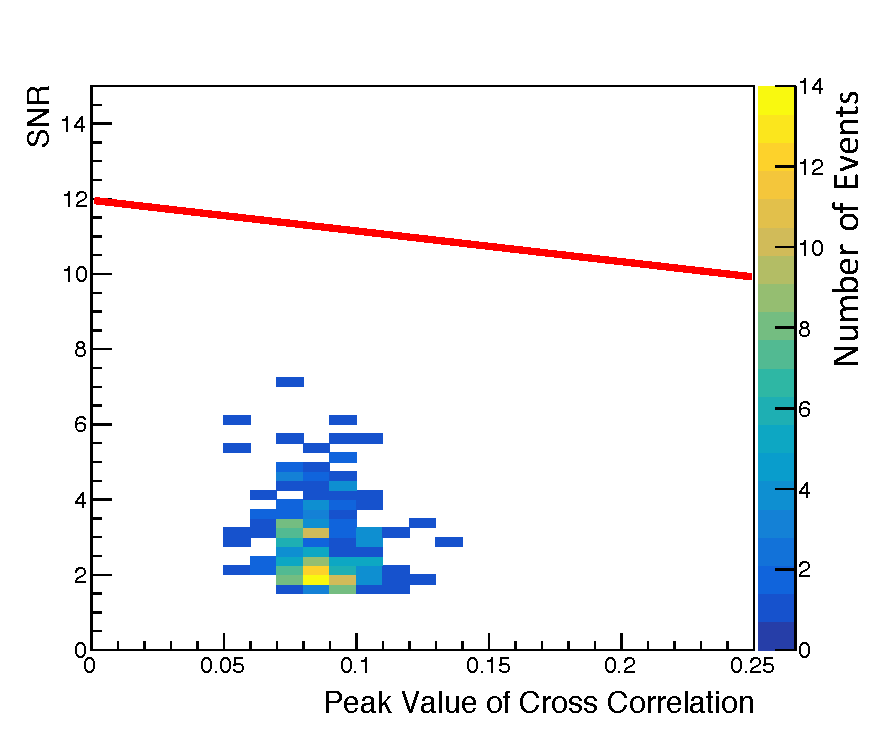
\includegraphics[width=0.65\textwidth]{figures/oindreeCorrSnrHist02970_175_439_V.pdf}
\par
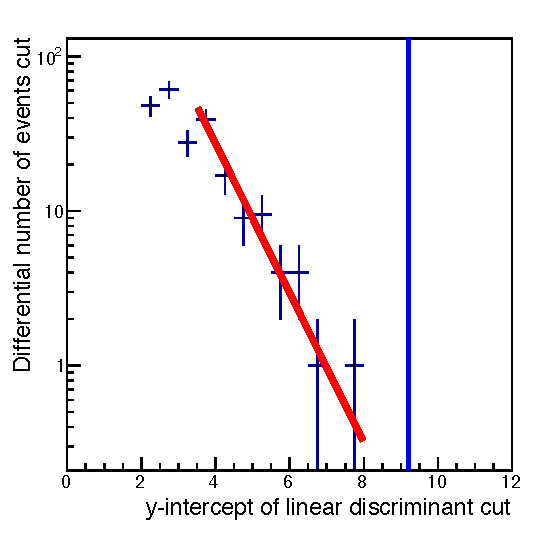
\includegraphics[width=0.65\textwidth]{figures/diffPlotVBin2970.pdf}
\caption{Top: The voltage SNR of the coherently summed waveform as a function of peak cross-correlation value for events in the 10\% dataset of the ANITA-3 binned analysis, reconstructing to Bin 2970, in the vertical polarization analysis. The red line shows the linear discriminant for this bin with an optimized slope. The y-intercept of this linear discriminant is not yet optimized. Bottom: The y-intercept associated with the events from Bin 2970 fit to an exponential. The vertical blue line shows the optimized LD cut for this bin.}
\label{bin2970}
\end{figure}


\subsubsection{Bin cut}

A bin is cut from the analysis if it does not meet certain requirements. 
In previous attempts of the binned analysis ~\cite{samStaffordThesis,jacobGordonThesis}, a bin was 
cut if it did not have five consecutive histogram bins with bin content values in descending order in the distribution of y-intercepts for a bin. As described in Chapter~\ref{results_diffuse}, this rule was later updated.
A distribution of y-intercepts is shown in the bottom plot of Figure~\ref{bin2970}. 
A bin was also cut if the exponential fit to the distribution of y-intercepts returned a bad p-value. 
A p-value less than 0.05 and greater than 0.999 was considered bad. 
In~\cite{samStaffordThesis,jacobGordonThesis}, a bin was rejected if the background estimate for that bin was greater than 1.0. This rule was also later updated as discussed in Chapter~\ref{results_diffuse}. 
Finally, bins with the lowest neutrino sensitivity, as derived from simulation, were also cut.
Neutrino sensitivity for a bin is estimated based on the number of simulated neutrinos that pass all cuts before the LD cut and reconstruct to that bin.  
More simulated neutrinos mean that area of the ice is more sensitive to neutrinos.  The least sensitive bins with cumulative sensitivity of less than 1\% (after all previous bin cuts) are removed for low sensitivity. These bins are used as a sideband in the analysis.

\subsubsection{Cut on events with a weight less than 0.5}

Events with an event weight of less than 0.5 are cut.  An event weight of less than 0.5 corresponds to the event being less than 50\% likely to have come from the Healpix bin it is seen passing in.  We want passing events to pass in the Healpix bin they are mostly within.


\section{The problem: Too many background events passing in the binned analysis}
\label{background_problem}

Reducing background events was one of the biggest priorities in the development of the binned analysis. The binned analysis was first tested using data from the \gls{anita}-2 flight. In this first pass at the binned analysis, it was found that too many events passed final cuts. In the \gls{vpol} channel of the analysis, 2.6 background events were expected to pass. Three isolated events were found to pass which was consistent with the background expectation. However, {\bf 21 excess} events were found to require a clustering cut at the end. Requiring a clustering cut at the end should ideally be avoided in the binned analysis which is principled on recovering ice that is deemed unusable by the clustering analyses. In total, {\bf 40 events} passed all cuts prior to the clustering cut, of which {\bf 24} were strong in \gls{vpol}, {\bf 26} in \gls{hpol} and {\bf 10} in both. Two of the 40 events were inserted, so the total number of background events to account for was {\bf 38}.

My goal was to remove such background events to consequently reduce analysis thresholds for the end goal of increasing sensitivity to neutrinos. This involved studying the data to obtain a deeper understanding of different classes of background. I started by focusing on the excess events passing in Bin 3045 of the \gls{anita}-2 binned analysis. This was the bin with the highest sensitivity in the \gls{anita}-2 binned analysis. Events passing all but the clustering cut {\bf and reconstructing} to this bin are summarized in Figure~\ref{bin3045}. The five events all took place on January 8, 2009 within minutes of each other.

\begin{figure}
\centering

\includegraphics[width=1.0\textwidth]{figures/bin3045_summary.png}
\caption{Summary of excess events passing in Bin 3045 of the ANITA-2 binned analysis.}
\label{bin3045}
\end{figure}

\begin{figure}
\centering
\subfloat[Bumps]{
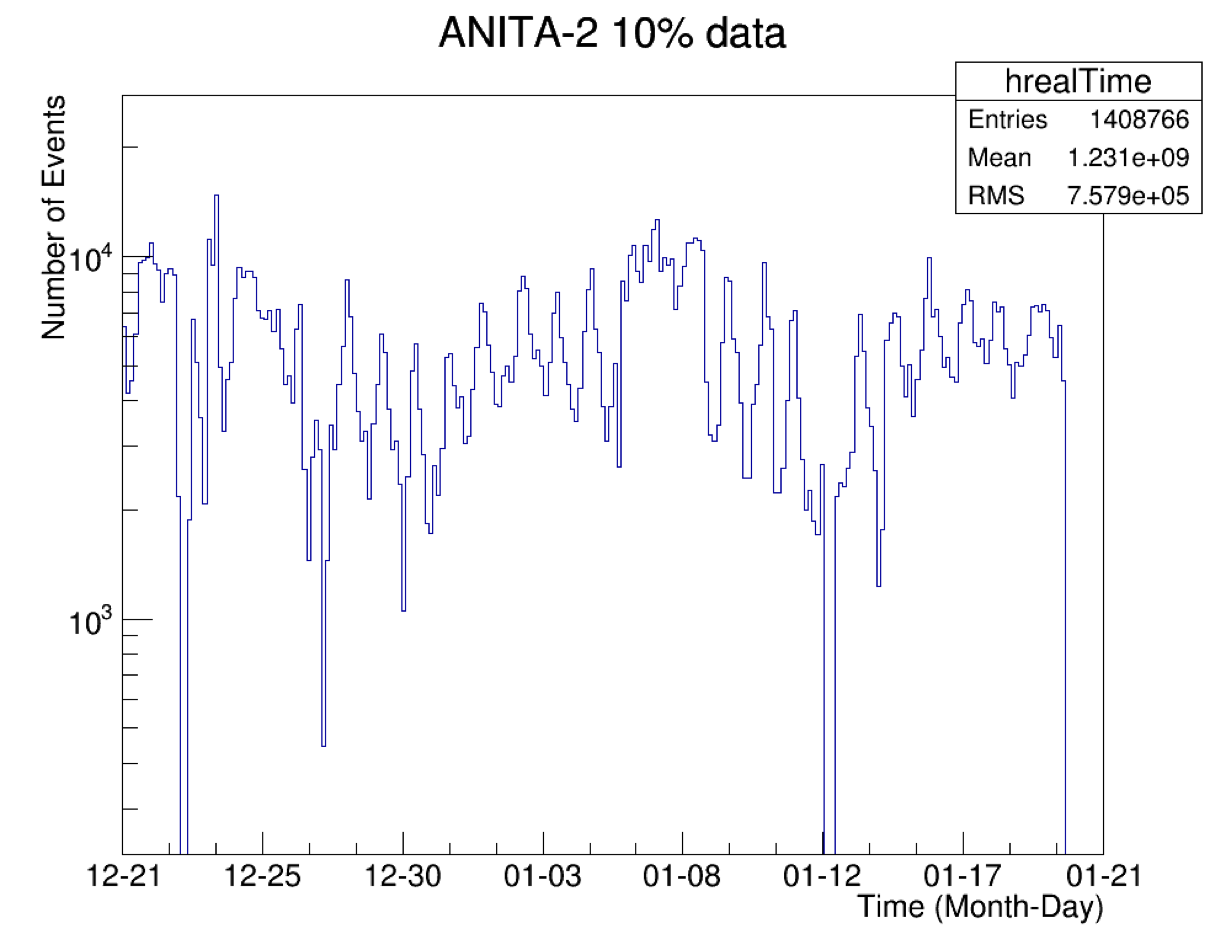
\includegraphics[width=0.8\textwidth]{figures/bumps_a2_full_flight.png}
\label{bumps}
} \par
\subfloat[FFT]{
\centering
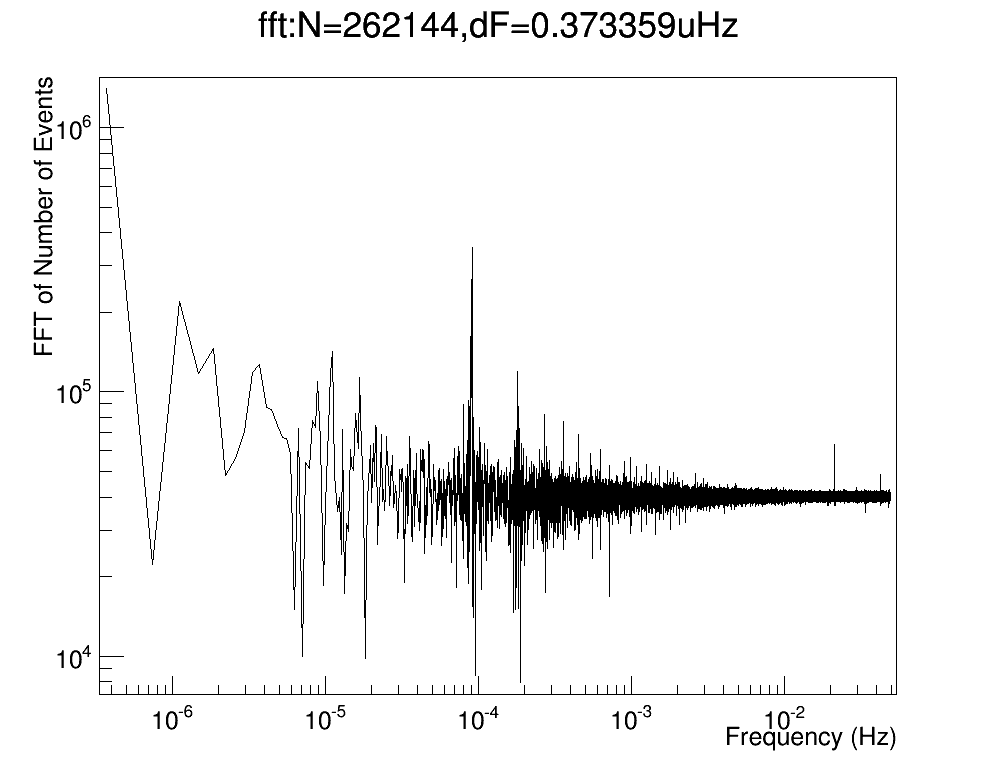
\includegraphics[width=0.8\textwidth]{figures/fullflightrealTimeFFT.png}
\label{fft_full}
}
\caption{Distribution of number of events as a function of time during the ANITA-2 flight (top) and the FFT of the same (bottom).}
\label{bumps_fft_full}
\end{figure}

\subsection{Fun with FFTs}
\label{fft}

I investigated the \gls{anita}-2 data for background that might appear at regular intervals of time and found bumps in the data throughout the flight as shown in Figure~\ref{bumps}. These bumps seemed to appear at a period of a day, by eye, which would correspond to about $>10^{-5}\,\mbox{Hz}$. I calculated the \gls{fft} of the full flight which is shown in Figure~\ref{fft_full}. The highest peak in the \gls{fft} is at $>10^{-4}\,\mbox{Hz}$. 

The \gls{anita} payload flew over Bin 3045 thrice during the \gls{anita}-2 flight. I calculated the \gls{fft} of the region in time for each pass of the payload over Bin 3045, including January 8 (which is when the excess events from Bin 3045 were recorded) region in time for events that reconstructed to Bin 3045 as shown in Figure~\ref{fft_jan8}. Interesting features were present in the \gls{fft}, one of which was accounted for by the removal of software triggered events from the data. Both a regularly triggered event and the removal of such events can cause peaks at the corresponding frequency in the \gls{fft}.

\begin{figure}
\centering
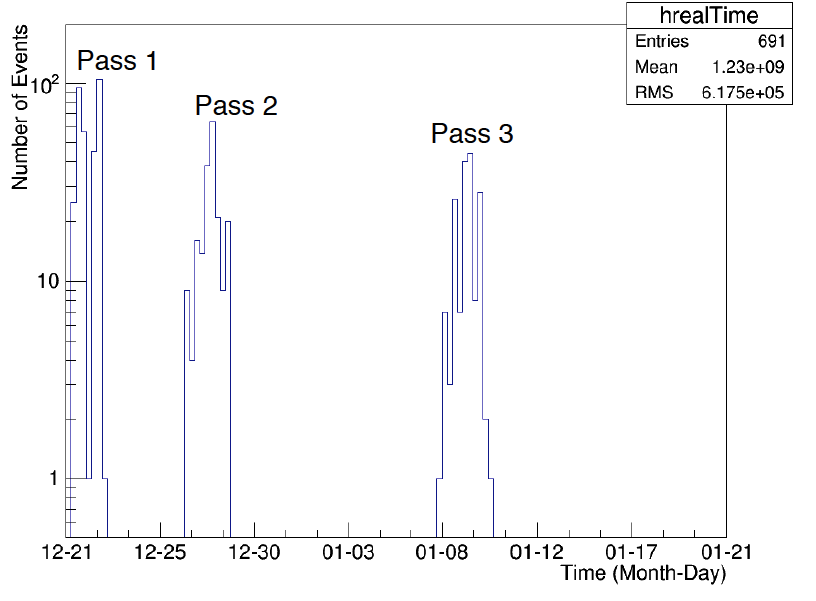
\includegraphics[width=0.8\textwidth]{figures/bin3045_3passes.png}
\caption{The three passes of the ANITA payload over Bin 3045 in the ANITA-2 binned analysis. }
\label{bin3045_3passes}
\end{figure}


\begin{figure}
\centering
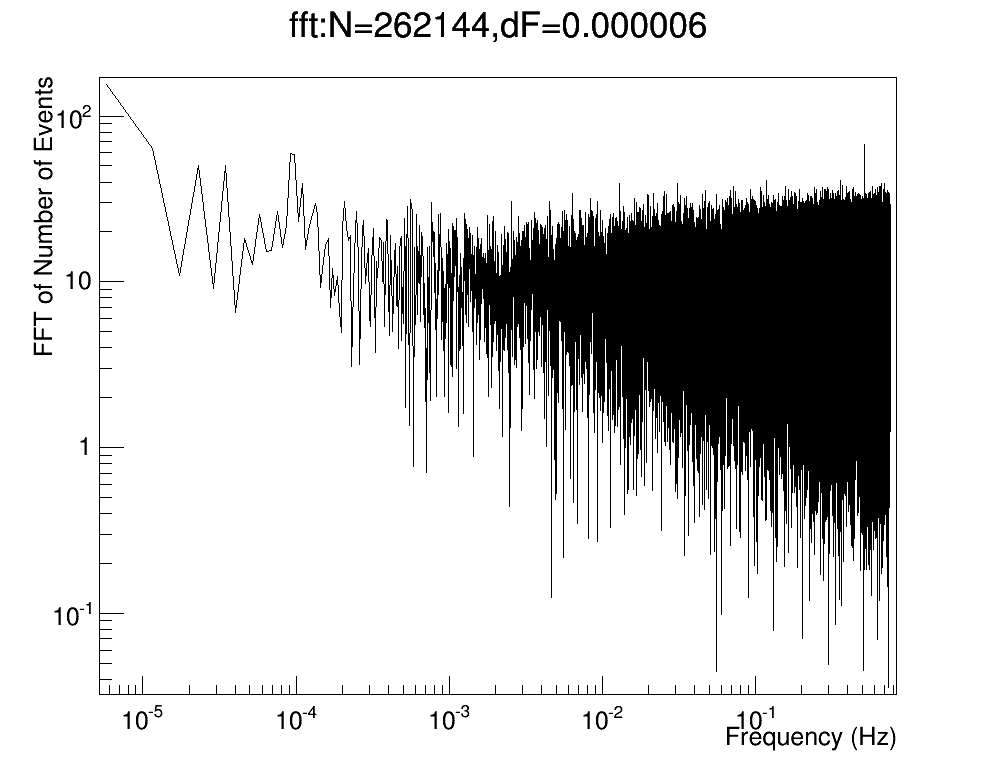
\includegraphics[width=0.8\textwidth]{figures/bin3045realTimeFFTJan8.png}
\caption{FFT of the January 8 region in time of the ANITA-2 flight for only events that reconstruct to bin 3045.}
\label{fft_jan8}
\end{figure}

\section{Satellite contamination}
\label{satellite}

We hypothesized that modulated \gls{cw} noise from satellites might have contributed to the events passing all but a clustering cut in Bin 3045 of the \gls{anita}-2 binned analysis. Reconstruction maps of these events are shown in Figure~\ref{bin3045cpolmaps}. We noted that the events were strong in \gls{hpol} as well as \gls{lcp} and \gls{rcp}. 

\subsection{Communication satellites}

There are numerous human-made satellites in orbit around the earth. Geosynchronous satellites have orbital period that matches earth's rotation on its axis, which takes one sidereal day of 23 hours 56 minutes and 4 seconds. Geostationary satellites have circular, geosynchronous equatorial orbits at 35,786 km
(22,236 mi) above the earth's equator and follow the direction of the earth's rotation. There are about a thousand geostationary satellites in orbit around the earth at the moment. Most communication satellites are geostationary. To a stationary observer on earth, the position of a geostationary satellite is fixed in the sky. 

Radio, \gls{cw} interference due to communication satellites, particularly military communication satellites, have been suspected to contribute to noise events for all \gls{anita} flights and particularly the \gls{anita}-3 flight. This is discussed further in Chapter~\ref{anita} Section~\ref{tuff}. We began to suspect that this effect might be seen as an over-density of events at certain longitudes as a function of the azimuthal angle of reconstruction of events. \gls{anita} has $360^{\circ}$ coverage in azimuth. Although geostationary satellites would be seen as fixed in the sky, the \gls{anita} payload itself moves. In fact, as \gls{anita} orbits over Antarctica, it traverses across all longitudes. Different geostationary satellites are present at different longitudes, and depending on the latitude of the payload, can be viewable by \gls{anita}.

\subsection{Satellite stripe plot}

I made the now-(in)famous ``satellite stripe plot" which is shown in Figure~\ref{satstripesa2}. In this plot, the longitude of the \gls{anita} payload is in the vertical axis and the azimuthal reconstruction angle of events using their waveforms in \gls{lcp} is in the horizontal axis. Note that the  quantity in the horizontal axis, phi, is {\bf corrected for heading} of the payload and calculated in ROOT as follows:

\begin{equation}
phi = fmod((phi_{LCP} - heading + 360),360)
\label{phi}
\end{equation}

The color axis represents the number of events with red indicating more events and blue indicating less events. Over-densities of events can be seen as stripes at certain longitudes, consistent with the hypothesis that satellites could be causing these. I made this plot first using data from the \gls{anita}-2 flight, and then also for \gls{anita}-3. Figure~\ref{stripes} shows the satellite stripe plot made using the 90\% data passing quality cuts from the \gls{anita}-2 flight on the left and the 10\% data passing quality cuts from the \gls{anita}-3 flight on the right. It can be seen that the {\bf same} stripes are present in the data from {\bf both} flights.

When events that had passed all but a clustering cut in the \gls{anita}-2 and \gls{anita}-3 binned analyses were overlaid on the corresponding satellite stripe plots, the plot thickened.
All five events passing in Bin 3045 in the \gls{anita}-2 binned analysis were on one of the stripes. 
In fact, {\bf 16 out of the 38} total non-inserted excess events that had passed all but the clustering cut in the \gls{anita}-2 binned analysis landed on top of these stripes. These are labeled in Figure~\ref{satstripesa2}. Five of the eight events that had passed in the binned analysis of the \gls{anita}-3 10\% data as reported in ~\cite{samStaffordThesis} were also on stripes.

\begin{figure}
\centering
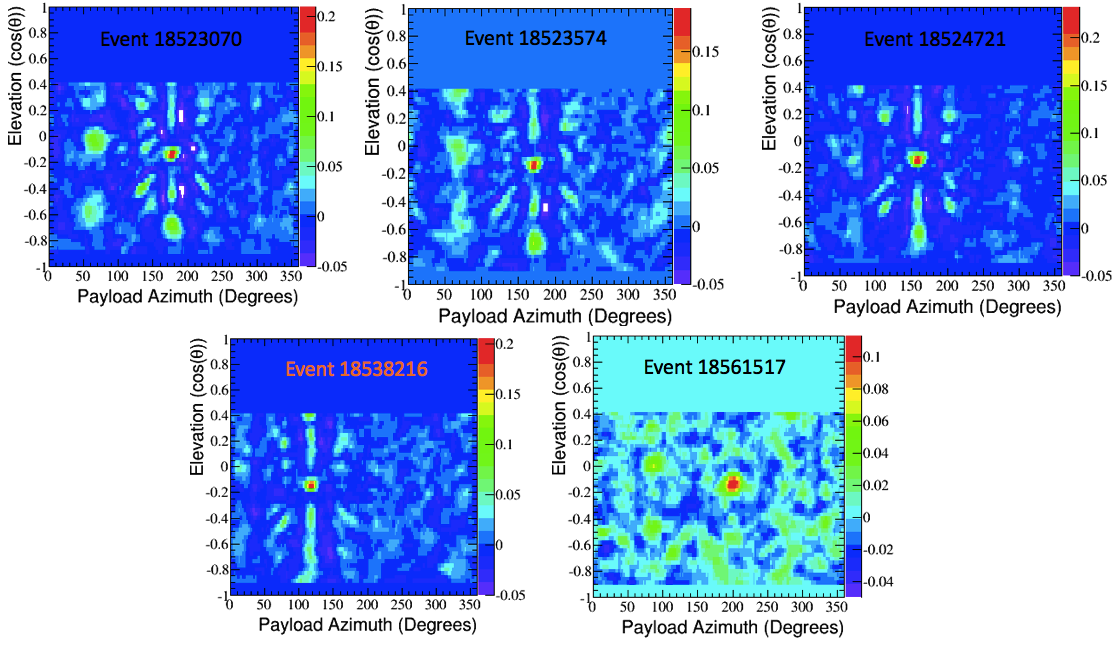
\includegraphics[width=1.0\textwidth]{figures/bin3045EventsCpolMaps.png}
\caption{Reconstruction maps of the events that passed all but a clustering cut in Bin 3045 of the ANITA-2 binned analysis. These maps are found using the left-circularly polarized waveforms of these events. That is the polarization associated with satellites.}
\label{bin3045cpolmaps}
\end{figure}

\begin{figure}
\centering
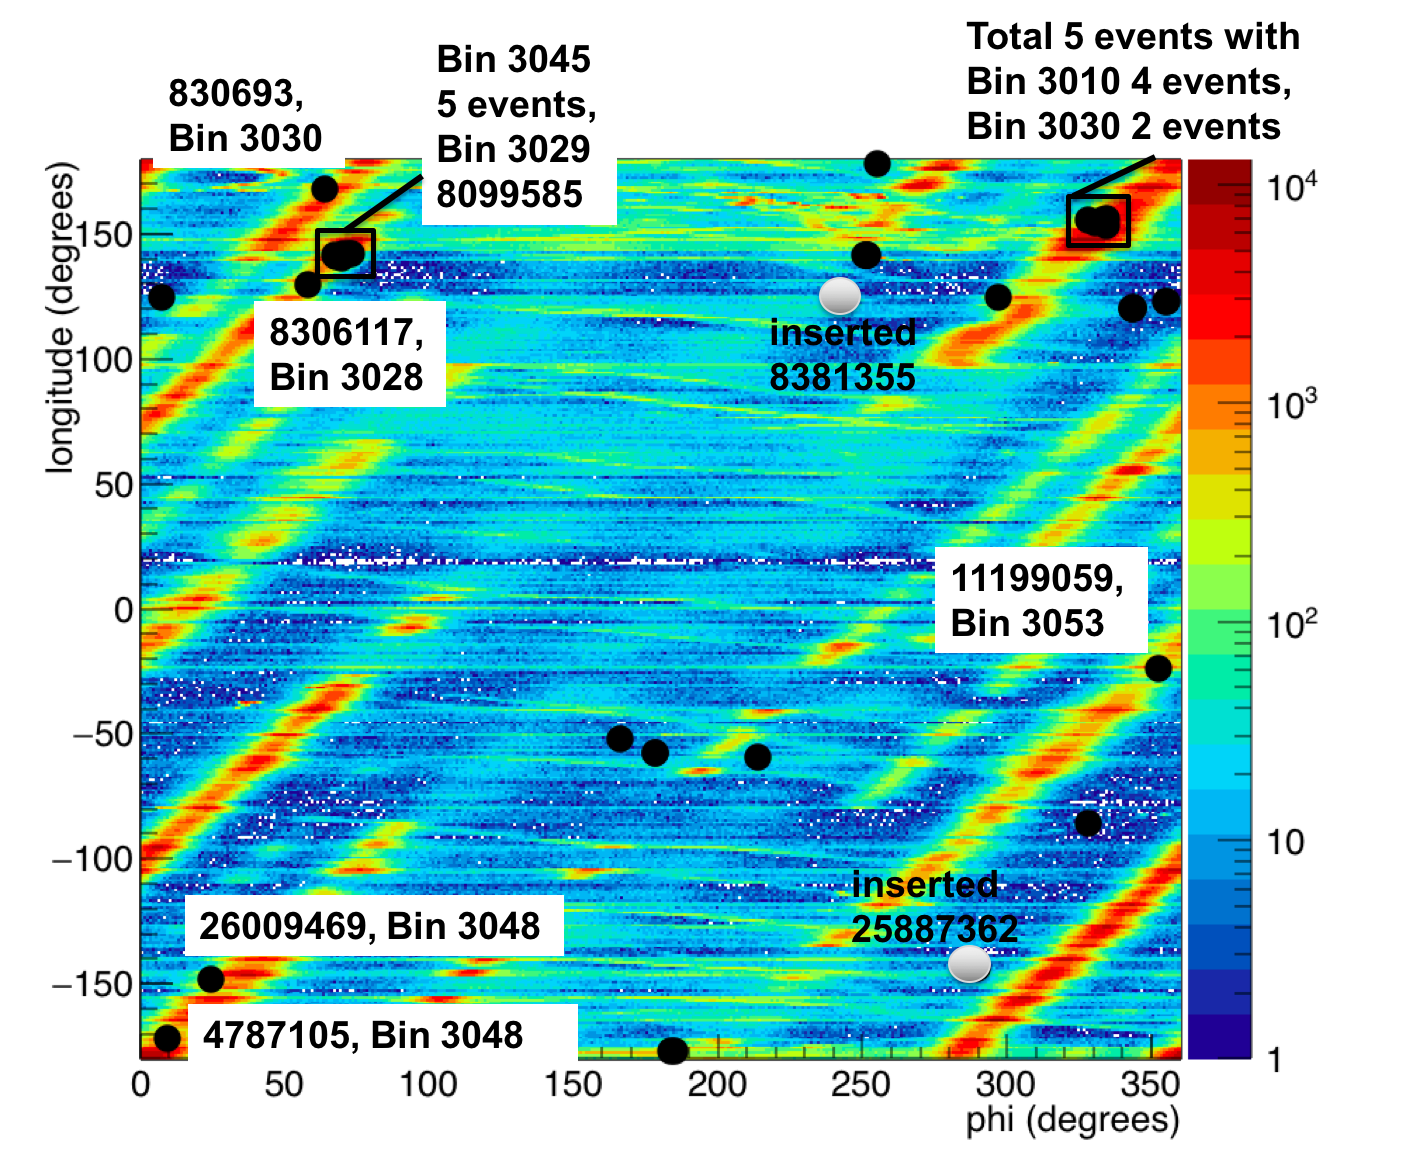
\includegraphics[width=1.0\textwidth]{figures/A2StripesSatInserted.png}
\caption{ANITA-2 satellite stripe plot with events labeled.}
\label{satstripesa2}
\end{figure}

\begin{figure}
\centering
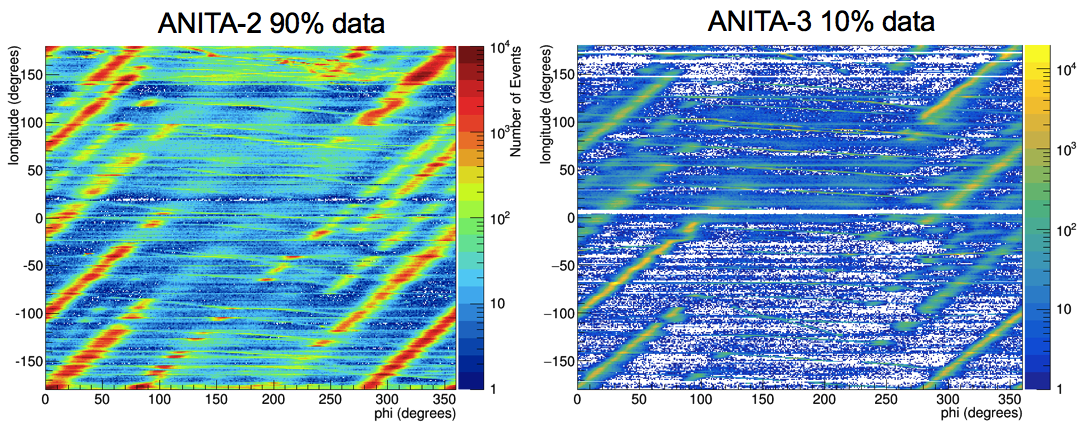
\includegraphics[width=1.0\textwidth]{figures/same_stripes.png}
\caption{Same stripes in both ANITA-2 and ANITA-3 flights.}
\label{stripes}
\end{figure}


\section{Satellite stripe cut}
\label{removing_sat}

Our goal was to reduce the number of events passing final cuts in the binned analysis that reconstructed to a satellite stripe. For this, it was necessary to determine equations for the upper and lower bound of each stripe. 

\subsection{Equations of Midlines}

Equations for lines denoting approximately the middle of each stripe, referred to as ``midlines", were determined as shown in Equation~\ref{midlines}. These are NOT the final equations used to implement the satellite stripe cut that we discuss in Section~\ref{stripe_eqn}, however, these midlines are the starting point in determining the final equations following the methods described in Section~\ref{sat_method}. 

\begin{align}
\begin{cases}
& stripe~1: longitude = phi -182.615 \\
& stripe~2: longitude = phi -100.435 \\
& stripe~3: longitude = phi -20.035 \\
& stripe~4: longitude = phi +32.81 \\
& stripe~5: longitude = phi +75.485 \\
& stripe~6: longitude = phi +101.3225 \\
\end{cases}
\label{midlines}
\end{align} 

\bigskip

In the above equations, longitude is the quantity in the vertical axis and phi is the quantity in the horizontal axis of Figures~\ref{satstripesa2} and \ref{stripes}. Again, note that the phi here is corrected for heading and given by Equation~\ref{phi}.

\subsection{Phi difference distribution}
\label{sat_method}

Using the relations in Equation~\ref{midlines}, cuts for the lower and upper bound of each stripe could be determined.
The phi in these equations is called the ``expected phi". 
A broader stripe was used that more than covered each stripe. In this broader stripe the difference between the phi of each event and the expected phi, that is, $phi - expected~phi$, was calculated. A distribution of this difference in phi and the expected phi, henceforth referred to as the ``phi difference distribution" was plotted for each stripe. This distribution for stripe 5 and using data from the \gls{anita}-2 flight is shown in Figure~\ref{phidist}. 

The left and right tail of each phi difference distribution was fit to a line which was subtracted off. This was meant to help reduce the continuum present in the distribution. Then each phi difference distribution was fit to a combination of gaussian functions. The equation for the fit as calculated using ROOT is shown in Equation~\ref{fit_gaus}. 

\begin{multline}
fit_{gauss} = [0]*exp(-(pow((x-[1]),2))/(2*pow([2],2))) + \\ [3]*exp(-(pow((x-[4]),2))/(2*pow([5],2))) + \\
[6]*exp(-(pow((x-[7]),2))/(2*pow([8],2))) 
\label{fit_gaus}
\end{multline}

\begin{figure}
\centering
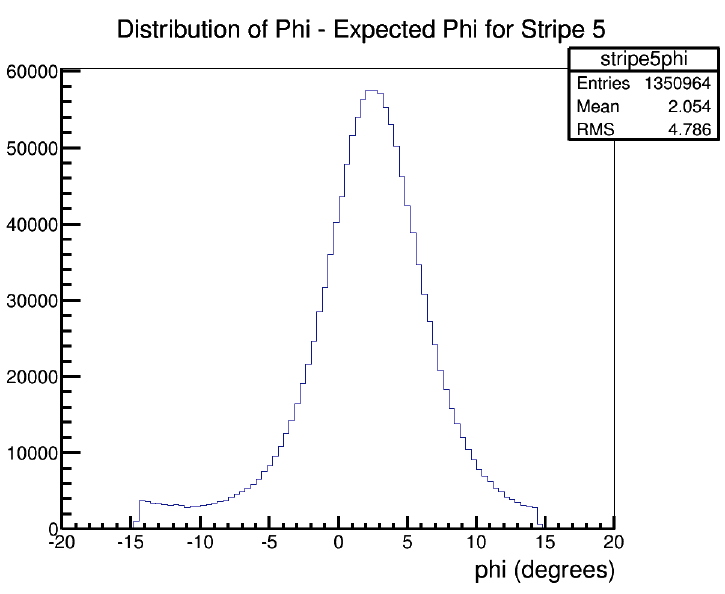
\includegraphics[width=0.8\textwidth]{figures/phi_dist_thesis.png}
\caption{Distribution of phi }
\label{phidist}
\end{figure}

For the \gls{anita}-3 analysis in ~\cite{diffuse,jacobGordonThesis}, cuts were chosen on the left and right tails of the fit to the phi difference distribution of each stripe using events just before the final LD cut. These events included a preliminary low LD cut given by: 

\begin{equation}
LD~cut > 4.0
\end{equation}

where the LD cut is calculated as follows:

\begin{equation}
LD~cut = cohSnr2 * (-6.0 ) + cPeak
\end{equation}
where cohSnr2 is the quantity in the vertical axis and cPeak is the quantity in the horizontal axis of Figure~\ref{bin2970}.

The cuts were chosen with the motivation to reduce the number of events passing that sit on a satellite stripe by a factor of 100. The cuts and the corresponding estimate on how many events should pass that sit on a stripe are presented in Table~\ref{sat_cuts}. It was found that stripes 5 and 6 actually needed to have sub-stripes that had to be cut rather than the entire stripe. The cut on the left side of the phi difference distribution fit is denoted as the ``left cut" while the cut on the right side of the phi difference distribution fit is denoted as the ``right cut". The number of events passing these cuts was also calculated to make sure it was consistent with only 1\% of events in the stripe.
Before the satellite stripe cut was implemented, roughly 100 events were expected to pass that would sit on stripes. This cut would allow a factor of 100 fewer or 1 event to pass that would sit on a stripe. 

\begin{center}
\begin{tabular}{ c c c c }
 Stripe name & Left cut & Right cut & Number of events passing \\
 Stripe 1  & -10.8  & 10.8  & 10.77 out of 988.67  \\ 
 Stripe 2  & -6.2   & 11.0  & 18.78 out of 1701    \\  
 Stripe 3  & -26.3  & -13.4 & 141.5 out of 13902    \\
 Stripe 4  & 26.5   & 39.3  & 135.6 out of 13754    \\
 Stripe 5a & -22.99 & -16.5 & 0.406 out of 34.263 \\
 Stripe 5b & -6.0   & 12.2  & 1.34 out of 139.57  \\
 Stripe 6a & 3.0    & 8.5   & 0.27 out of 31.197 \\
 Stripe 6b & 23.2   & 32.8  & 0.93 out of 93.086
\end{tabular}
\label{sat_cuts}
\end{center}

\subsection{Equations for stripes}
\label{stripe_eqn}

Combining the cuts in Table~\ref{sat_cuts} with the equations of midlines in Equation~\ref{midlines}, we obtained equations for lines for the lower and upper bound of each stripe. These are shown in Equations~\ref{cut_lines} and ~\ref{cut_lines2}.

\begin{align}
\begin{cases}
&  Stripe~1~upper: longitude = phi - 171.815 \\
&  Stripe~1~lower: longitude = phi - 193.415 \\
&  Stripe~2~upper: longitude = phi - 89.435 \\
&  Stripe~2~lower: longitude = phi - 106.635\\
&  Stripe~3~upper: longitude = phi - 33.435\\
&  Stripe~3~lower: longitude = phi - 46.335\\
&  Stripe~4~upper: longitude = phi + 72.11\\
&  Stripe~4~lower: longitude = phi + 59.31\\
\end{cases}
\label{cut_lines}
\end{align}

\begin{align}
\begin{cases}
&  Stripe~5a~upper: longitude = phi + 58.985\\
&  Stripe~5a~lower: longitude = phi + 52.495\\
&  Stripe~5b~upper: longitude = phi + 87.685\\
&  Stripe~5b~lower: longitude = phi + 69.485\\
&  Stripe~6a~upper: longitude = phi + 109.823\\
&  Stripe~6a~lower: longitude = phi + 104.323\\
&  Stripe~6b~upper: longitude = phi + 134.123\\
&  Stripe~6b~lower: longitude = phi + 124.523\\
\end{cases}
\label{cut_lines2}
\end{align}

We wanted to recover some events within stripes utilizing the property that satellite-contaminated events were thought to have larger peak value of cross-correlation in \gls{lcp} than in \gls{rcp}. 
Therefore, within a stripe we required the condition that the peak value of cross-correlation in \gls{rcp} divided by that in \gls{lcp} had to be greater than some number.
These numbers were chosen by trying different cuts on the ratio of \gls{rcp}/\gls{lcp} that made the phi difference distributions of the stripes flatter. The final numbers are shown in Equation~\ref{ratio}. 

\begin{align}
\begin{cases}
Stripe~1: \frac{Peak_{RCP}}{Peak_{LCP}} = 1.7\\
Stripe~2: \frac{Peak_{RCP}}{Peak_{LCP}} = 2.2\\
Stripe~3: \frac{Peak_{RCP}}{Peak_{LCP}} = 2.2\\
Stripe~4: \frac{Peak_{RCP}}{Peak_{LCP}} = 1.7\\
Stripe~5: \frac{Peak_{RCP}}{Peak_{LCP}} = 2.0\\
Stripe~6: \frac{Peak_{RCP}}{Peak_{LCP}} = 2.0\\
\end{cases}
\label{ratio}
\end{align}


\begin{table}
\centering
\begin{tabular}{ |c|c|c|c|c|c|c| } 
\hline
Flight & Analysis & Dataset & Analyst & Excess events & Num. on stripes & \% \\
\hline
ANITA-2 & Diffuse & 90\% & B. Dailey & 38 & 16 & 42\%\\
ANITA-3 & Diffuse & 10\% & S. Stafford & 9 & 6 & 67\%\\
\hline
\end{tabular}
\caption{Summary of results motivating the satellite stripe cut.}
\label{stripe_cut}
\end{table}


\subsection{Summary and impact}

The satellite stripe cut was developed to mitigate the problem of excess events passing final cuts in previous attempts of the binned analysis to search for a diffuse flux of \gls{uhe} neutrinos in data from the \gls{anita}-2 and -3 flights. A large fraction of the excess events were on the satellite stripes as summarized in Table~\ref{stripe_cut}. This led to the hypothesis that satellites in orbit around the earth could be causing anthropogenic noise lined up with the satellites in azimuth to pass the trigger and get recorded as data by \gls{anita}. These satellites could be causing events to pass our analysis cuts too without a satellite stripe cut in place. The excess events showing up as stripes in Figures~\ref{satstripesa2} and~\ref{stripes} support this hypothesis and imply that most of the \gls{anita} triggered events are actually along stripes and satellite-contaminated. 

The goal of the satellite stripe cut was to remove satellite-contaminated events from the dataset. Upon implementation, the stripe cut removed 69\% of events (after a few quality cuts) in the \gls{anita}-3 data, dramatically reducing the dataset. The price paid was that 17.8\% of simulated neutrinos were also lost due to this cut. Events in viewing gaps expected for satellites at 0 degrees with respected to the equator were retained. The name of the function used to do this is \path{canANITASeeStripe}. 

The problem with satellite contamination was deemed severe enough to implement this overall harsh cut. However, in the future, the satellite stripe cut could be implemented with certain modifications such as taking into account the reconstructed azimuthal direction of events and retaining events that produced triggers on a side of the payload that is not facing the satellites.